% ============================================================================
% Accessibility
% ============================================================================
\DocumentMetadata{
  lang = en-US, 
  pdfstandard = ua-2, 
  tagging = on, 
  tagging-setup = {math/setup=mathml-SE}
}

% ============================================================================
% Document Properties - used on title slide and PDF metadata fields
% ============================================================================
\def\PresTitle{Gauge Blocks}  % Required - top line of title slide
\def\PresSubtitle{Gauges and Measurement}         % Optional - second line
\def\PresAuthor{Brad Peirson}               % Required - below dividing line
\def\PresInstitute{College of Information Technology and Engineering}       % Optional
\def\PresDate{}                             % Optional
\def\PresKeywords{}                         % Optional - used for hyperref

% Presentation Formatting
% ============================================================================
% ============================================================================
% Class Declaration
% ============================================================================
\documentclass[
        mode = handout,     % Projector = one bullet at a time, Handout = all
        font-size=14pt,     % Only accepts 9, 10, 12, 14, 17, 20
        pdfusetitle         % Pulls \title property from document
    ]
    {ltx-talk}              % ltx-talk class

% ============================================================================
% Custom Colors
% ============================================================================
\usepackage[table]{xcolor}
% Colors from the Baker College Style Guide
%\definecolor{BakerADARed}{RGB}{231, 0, 46}   % #e7002e Official ADA red-doesn't pass WCAG AAA for small text
\definecolor{BakerADARed}{RGB}{181, 0, 36}    % #b50024 Adjusted ADA red-passes WCAG AAA for small text
\definecolor{HoneyYellow}{RGB}{255, 196, 0}   % #ffc400
\definecolor{UpNorthGreen}{RGB}{114, 191, 68} % #72bf44
\definecolor{LakeBlue}{RGB}{134, 183, 227}    % #86b7e3
\definecolor{BakerADI}{RGB}{58, 98, 170}
\definecolor{BakerCIM}{RGB}{217, 35, 47}
\definecolor{BakerBlack}{RGB}{31, 34, 40}     % #1f2228
\definecolor{BakerWhite}{RGB}{255, 255, 255}
\definecolor{BakerRed}{RGB}{239, 0, 48}
\definecolor{Abbey}{RGB}{80, 82, 88}
\definecolor{RollingStone}{RGB}{121, 124, 126}
\definecolor{HitGray}{RGB}{165, 169, 172}
\definecolor{Iron1}{RGB}{201, 206, 209}
\definecolor{Iron}{RGB}{222, 225, 226}
\definecolor{BlackHaze1}{RGB}{237, 240, 240}
\definecolor{BlackHaze}{RGB}{245, 247, 247}

% ============================================================================
% Document Data
% ============================================================================
\title{\PresTitle}
\author{\PresAuthor}
\institute{\PresInstitute}
\date{\PresDate}

%Set up the hyperlink colors
\hypersetup{colorlinks,
    linkcolor=BakerBlack,
    urlcolor=BakerADARed,
    pdfauthor = {\PresAuthor},
    %pdftitle = {\PresentationTopic},   % Title is pulled directly
    pdfsubject = {\PresSubtitle},
    pdfkeywords = {\Keywords},
    pdfcreator = {LaTeX with hyperref package},
    pdfproducer = {LuaLaTeX}
    }

% Map your custom style guide colors to the progress bar aliases
\colorlet{pbcomplete}{BakerADARed}
\colorlet{pbincomplete}{Iron}

\usepackage[most]{tcolorbox}

% ============================================================================
% Footer Format
% ============================================================================
\EditInstance{footer}{std}{
  color         = Abbey,
  separator     = \hfill,
  element-order = {title, institute, framenumber},
  right-hspace  = 3mm,
  left-hspace   = 3mm,
}

% \DeclareInstance{footer}{empty}{
%   element-order = {}
% }

% ============================================================================
% Progress Bar Toggles & Helper Macros
% ============================================================================
\usepackage{xfp}        % Needed for floating point math
\newif\ifprogressbar    % Used to determine whether or not to show the bar
\progressbartrue        % Set the bar to true at the start

% Helper macro to automatically turn off the progress bar inside title/section frames
\newcommand{\makeblindframe}[1]{%
  \progressbarfalse
  #1%
  \progressbartrue
}

% ============================================================================
% Custom Page Formats
% ============================================================================
\let\oldmaketitle\maketitle         % Backup the original maketitle command
\let\oldsection\section             % Backup the original section command
\let\oldsubsection\subsection       % Backup the original subsection command

\makeatletter
\renewcommand{\maketitle}{%
\makeblindframe{%
  \disableglobalbackground
  \slidebackground{PresentationTitleGraphic_2048x1151}%
  \color{white}%
  %\UseInstance{footer}{wallpaper}
  \begin{frame}[wallpaper]
    \vspace*{1in}%
      \begin{tcolorbox}[
          enhanced,
          colback=black,       
          colframe=black,      
          opacityfill=0.25,       
          arc=6pt,                
          boxrule=0pt,            
          left=20pt, right=20pt,  
          top=20pt, bottom=20pt,
          width=0.80\textwidth,   
          halign=left             
      ]
          \color{white}%
          % Title (Always visible)
          {\large\bfseries\sffamily \@title}\\[0.5em]%
          
          % Conditional Subtitle
          \ifx\PresSubtitle\empty
          \else
            {\normalsize\sffamily \PresSubtitle}\\[0.5em]%
          \fi
          
          % High-contrast divider line
          {\color{white!80}\rule{0.3\textwidth}{0.8pt}}\\[0.5em]%
          
          % Author (Always visible)
          {\small\sffamily \@author}\\%
          
          % Conditional Institute
          \ifx\PresInstitute\empty
          \else
            {\small\sffamily \PresInstitute}\\%
          \fi
          
          % Conditional Date
          \ifx\PresDate\empty
          \else
            {\small\sffamily \@date}\\%
          \fi
      \end{tcolorbox}%
      \vfill     
  \end{frame}%
  \enableglobalbackground{BG}%
  \color{black}%
  %\UseInstance{footer}{std}
}%
}
\makeatother

% Create a variable container to hold the current section title
\newcommand{\currentsectiontitle}{}

% Redefine \section to take 1 argument (the title)
\renewcommand{\section}[1]{%
\makeblindframe{%
  \renewcommand{\currentsectiontitle}{#1}%
  \disableglobalbackground
  \slidebackground{PresentationSectionBackground_2048x1151}%
  \begin{frame}
    \vfill
    %\vspace*{0.625in}%
    \begin{tcolorbox}[
        enhanced,
        colback=black,       
        colframe=black,      
        opacityfill=0.25,       
        arc=6pt,                
        boxrule=0pt,            
        left=20pt, right=20pt,  
        top=20pt, bottom=20pt,
        width=0.80\textwidth,   
        halign=left             
    ]
        \color{white}%
        {\large\bfseries\sffamily #1}\\[0.5em]%   
    \end{tcolorbox}%
    \vfill 
  \end{frame}%
  \oldsection{#1}%
  \enableglobalbackground{BG}%

  % This will be used for an auto TOC at every section
  % Right now ltx-talk TOC is still in development
  % Once it comes a little further along this can be used
  % \begin{frame}
  %       \frametitle{Section Overview}
  %       \tableofcontents[sections=\thesection]
  %   \end{frame}%
}%
}

% Redefine \subsection to take 1 argument
\renewcommand{\subsection}[1]{%
\makeblindframe{%
  \disableglobalbackground
  \slidebackground{PresentationSectionBackground_2048x1151}%
  \begin{frame}
    \vfill
    %\vspace*{0.25in}% 
    \begin{tcolorbox}[
        enhanced,
        colback=black,       
        colframe=black,      
        opacityfill=0.25,       
        arc=6pt,                
        boxrule=0pt,            
        left=20pt, right=20pt,  
        top=20pt, bottom=20pt,
        width=0.80\textwidth,   
        halign=left             
    ]
        \color{white}%
        {\large\bfseries\sffamily\currentsectiontitle}\\[0.5em]%
        {\normalsize\sffamily #1}%
    \end{tcolorbox}%
    \vfill 
  \end{frame}%
  \oldsubsection{#1}%
  \enableglobalbackground{BG}%
}%
}

%Set the fonts to use NeueHaas Grotesk
\setsansfont{NHAASGROTESKTXPRO-}[
    Path=../NeueHaasGroteskFiles/,
    Scale=1.0,
    Extension = .ttf,
    UprightFont=*55Rg,
    BoldFont=*75Bd,
    ItalicFont=*56It,
    BoldItalicFont=*76BdIt
    ]

% Force the document default family to Sans-Serif
\renewcommand{\familydefault}{\sfdefault}

\usepackage{mathtools} % Load BEFORE unicode math settings
\setmathfont{Fira Math}[Scale=MatchLowercase] 

% 1. Turn global background ON
\newcommand{\enableglobalbackground}[1]{%
  \AddToHook{shipout/background}[mybg]{%
    \put(0, -\paperheight){%
      \includegraphics[width=\paperwidth, height=\paperheight, artifact]{#1}%
    }%
  }%
}

% 2. Turn global background OFF
\newcommand{\disableglobalbackground}{%
  \RemoveFromHook{shipout/background}[mybg]%
}

\newcommand{\slidebackground}[1]{%
  \AddToHookNext{shipout/background}{%
    \put(0, -\paperheight){%
      \includegraphics[width=\paperwidth, height=\paperheight, artifact]{#1}%
    }%
  }%
}

% --- GLOBAL BULLET OVERRIDES ---
\renewcommand{\labelitemi}{\color{BakerBlack}\Large\textbullet}
\renewcommand{\labelitemii}{\color{BakerBlack}\large\textbullet}
\renewcommand{\labelenumi}{\color{BakerBlack}\bfseries\arabic{enumi}.}
\renewcommand{\labelenumii}{\color{BakerBlack}\bfseries\alph{enumii})}

\AddToHook{begindocument/before}{%
  \EditInstance{item}{description}{
    label-format = \normalfont\bfseries\color{BakerADARed}#1
  }%
}

\AddToHook{begindocument/before}{%
  \EditInstance{item}{basic}{
    label-format = \color{BakerADARed}#1
  }%
}

% Global override for ltx-talk slide titles
\EditInstance{frametitle}{header}{
    font = \rule{0pt}{1.5cm}\bfseries\Large,
}

\EditInstance{header}{std}{
    font = \bfseries\huge,
    color = BakerBlack,
}

\AddToHook{env/block/begin}{%
  \colorlet{structure}{BakerADARed}%
}

\pretocmd{\tableofcontents}{\begin{minipage}{\textwidth} \linespread{1.4}}{}{}
\apptocmd{\tableofcontents}{\end{minipage}}{}{}

%Biber not functional in ltx-talk as of 2026-05-29
%Package that allows the creation of bibliographies
\usepackage[
    backend=biber,
    style=authoryear,
    sorting=none,
    %entryhead=false
    ]{biblatex}

%Load the bibliography file
\addbibresource{../../reference.bib}

\defbibheading{bibslide}{References}

\newcolumntype{L}[1]{>{\raggedright\let\newline\\\arraybackslash\hspace{0pt}}m{#1}}
\newcolumntype{C}[1]{>{\centering\let\newline\\\arraybackslash\hspace{0pt}}m{#1}}
\newcolumntype{R}[1]{>{\raggedleft\let\newline\\\arraybackslash\hspace{0pt}}m{#1}}

%All of the graphics are in a seperate folder, this makes it so the folder doesn't have to be repeated every time
\graphicspath{
  {../assets/images}
  {../assets/diagrams}
  {../assets/plots}
}

\makeatletter
% New counter to hold the custom "max frames" for the progress bar
\newcommand{\pb@maxtotal}{1}

% Read the custom total from the .aux file if it exists
\AtBeginDocument{%
  \ifdefined\pb@storedtotal
    \let\pb@maxtotal\pb@storedtotal
  \else
    % Fallback to standard total if our custom hook hasn't run yet
    \edef\pb@maxtotal{\@totalframes}%
  \fi
}

% Custom Appendix command that caps the progress bar and turns it off
\newcommand{\talkappendix}{%
  % 1. Write the CURRENT frame number to the .aux file as the progress total
  \immediate\write\@auxout{\string\gdef\string\pb@storedtotal{\@framenumber}}%
  % 2. Turn off the progress bar for all subsequent appendix slides
  \progressbarfalse
}
\makeatother

% ============================================================================
% Progress Bar Logic 
% ============================================================================
\makeatletter               
\AddToHook{shipout/background}{%
  \ifprogressbar
    % Read ltx-talk's internal frame counter safely
    \edef\currentframe{\@framenumber}%
    \edef\totalframes{\pb@maxtotal}% Use our custom max total instead
    
    % Fallback checks: If the document hasn't fully compiled yet, default to 1
    \ifx\currentframe\empty\def\currentframe{1}\fi
    \ifx\totalframes\empty\def\totalframes{1}\fi
    
    % Draw the progress bar if we have a valid total frame count
    \ifnum\totalframes>1\relax
      % Compute fraction width: (current - 1) / (total - 1)
      \edef\pbfraction{\fpeval{(\currentframe - 1) / (\totalframes - 1)}}%
      
      % Guard rails to prevent the bar from overshooting 100% on a first compile
      \ifdim\pbfraction pt>1pt\def\pbfraction{1}\fi 
      
      \edef\completewidth{\fpeval{\pbfraction * \paperwidth}}%
      \edef\incompletewidth{\fpeval{\paperwidth - \completewidth}}%
      
      % Render full-width progress bar at the top edge
      \put(0cm, -0.1cm){%
        \color{pbcomplete}\rule{\completewidth pt}{2pt}%
        \color{pbincomplete}\rule{\incompletewidth pt}{2pt}%
      }%
    \fi
  \fi
}
\makeatother

% 1. Globally shrink all caption components right as the caption engine fires
\AddToHook{cmd/@makecaption/before}{\footnotesize}

% 2. Declare and assign a blank plug to the kernel's caption label socket
\NewSocketPlug{caption/label}{nolabel}{}
\AssignSocketPlug{caption/label}{nolabel}

\usepackage{adjustbox}

\usepackage{amssymb}
\usepackage{amsmath}

\usepackage{animate}

\usepackage{calc} % Optional, but helpful for layout

\usepackage{multirow}

\usepackage{textcomp}

\usepackage[americanvoltages]{circuitikz}
\usepackage{pgfplots}
\usepackage{pgf-pie}

\usetikzlibrary{
    intersections, 
    fillbetween,
    patterns,
    decorations.pathreplacing,
    decorations.pathmorphing,
    decorations.text,
    decorations.markings,
    arrows.meta,
    arrows,
    shapes,
    shapes.geometric,
    shadows,
    calligraphy,
    backgrounds,
    intersections,
    calc,
    math,
    positioning,
    svg.path,
    shadows,
    shadows.blur
    }

\pgfplotsset{compat=1.18}

\pgfdeclarelayer{ft}
\pgfdeclarelayer{bg}
\pgfsetlayers{bg, main, ft}

% Usage: \hexpic[]{height}{Alt text}{Attribution}{image path}
\newcommand{\hexpic}[5][]{%
  \begin{figure}
    \centering
    \begin{tikzpicture}[
      baseline=(hex.base),      
      every shadow/.style={
        shadow opacity=70
        }
      ]
      \node (hex) [
        draw=white, 
        minimum size=#2, 
        regular polygon, 
        regular polygon sides=6, 
        rotate=90,
        blur shadow
      ] {};
      \begin{scope}
        \clip (hex.corner 1) -- (hex.corner 2) -- (hex.corner 3) -- 
              (hex.corner 4) -- (hex.corner 5) -- (hex.corner 6) -- cycle;
        \node at (hex.center) [#1] {
          \includegraphics[height=#2, alt={#3}]{#5}
        };
      \end{scope}
    \end{tikzpicture}

    \vspace{0.5em}
    {\tiny #4\par}
  \end{figure}  
}

% Usage: \shadowpic[]{width}{Alt text}{Attribution}{image path}
\newcommand{\shadowpic}[5][]{%
  \begin{figure}
    \centering
    \begin{tikzpicture}
      [every shadow/.style={
        shadow opacity=70
        }
      ]
      \node (image) [
        inner sep=0,
        blur shadow
      ] {\includegraphics[width=#2, alt={#3}]{#5}};
    \end{tikzpicture}

    \vspace{0.5em}
    {\tiny #4\par}
  \end{figure}
}

\tikzset{middlearrow/.style={
        decoration={markings, 
        mark= at position 0.5 with {\arrow{#1}},
        },
        postaction={decorate}
    }
}

% Usage: \tikztodo[width]{height}{description/notes}
\newcommand{\tikztodo}[3][0.8\textwidth]{%
  \begin{center}
    \fbox{%
      \parbox[c][#2][c]{#1}{%
        \centering
        \textbf{\textcolor{red}{TODO: TikZ Diagram}}\\[0.5em]
        \small #3%
      }%
    }%
  \end{center}%
}

% Macro: \drawrails{<number_of_1cm_segments>}
\newcommand{\drawrails}[1]{
  % Calculate total depth: 1 cm per segment
  \pgfmathsetmacro{\railheight}{-1 * #1}
  
  % L1 Rail (x = 0)
  \draw[thick] (0, 0) -- (0, \railheight cm);
    
  % L2 Rail (x = 15)
  \draw[thick] (15, 0) -- (15, \railheight cm);
}

\newcommand{\ccwplus}{%
  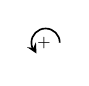
\begin{tikzpicture}[baseline=(char.base)]
    \node(char) at (0,0) {\(\scriptscriptstyle +\)};
    \draw[->, >=stealth, semithick] (0.2,0) arc (0:230:0.18cm);
  \end{tikzpicture}%
}

%====================================================================================
% Timer Ladder Symbol - Could be used for TON, TOF, RTO....
%====================================================================================
\tikzset{
    TON/.pic={

        \draw[
          BakerBlack
        ]
        (0,0)
        -- ++(0,0.375)
        -- ++(3.5,0)
        coordinate[pos=0.5](-TOP)
        -- ++(0,-1.75)
        coordinate[pos=3/14](-OUT)
        coordinate[pos=0.5](-EN1)
        coordinate[pos=0.875](-DN1)
        -- ++(-3.5,0)        
        -- (0,0)
        coordinate(-IN);

        \node[
          text=BakerBlack,
          font=\bfseries,
          anchor=east
        ](pre)
        at ($(-TOP)-(0,1.75em)$)
        {{\small PRE:}};

        \node[
          text=BakerBlack,
          font=\bfseries,
          anchor=east
        ](acc)
        at ($(pre.east)-(0,1em)$)
        {{\small ACC:}};

        \coordinate (-PRE) at (pre.east); % For the preset value
        \coordinate (-ACC) at (acc.east);

        \draw[
            BakerBlack
        ]
        (-EN1)
        -- ++(0.5,0)
        coordinate(-EN2)
        node[
            text=BakerBlack,
            anchor=west
        ]
        {{\small EN}};

        \draw[
            BakerBlack
        ]
        (-DN1)
        -- ++(0.5,0)
        coordinate(-DN2)
        node[
            text=BakerBlack,
            anchor=west
        ]
        {{\small DN}};

    }
}

%====================================================================================
% Oval ladder symbol, good for ONS, RES, etc.
%====================================================================================
\tikzset{
    ONS/.pic={

        \draw[
          BakerBlack
        ]
        (0,0)
        coordinate(-IN)
        -- ++(0.75,0)
        node[
          draw=BakerBlack, 
          text=BakerBlack, 
          font=\small, 
          minimum width=1.5cm, 
          minimum height=0.75cm, 
          anchor=west, 
          rounded corners=0.25cm
          ](ons){};
        
        \draw[BakerBlack] (ons.east) -- ++(0.75,0) coordinate(-OUT);

        \coordinate(-INS) at (ons.center);
        \coordinate(-VAR) at (ons.north); 
    }
}

%====================================================================================
% Source A, Source B, Dest box
%====================================================================================
\tikzset{
    SrcDest/.pic={
      
        \draw[
          BakerBlack
        ]
        (0,0)
        coordinate(-IN)
        -- ++(0,0.375)
        -- ++(5,0)
        coordinate[pos=0.5](-TOP)
        -- ++(0,-3.25)
        coordinate[pos=3/26](-OUT)
        -- ++(-5,0)
        -- (0,0)
        coordinate(l1);

        \node[
          text=BakerBlack,
          font=\bfseries,
          anchor=west
        ](srcA)
        at (l1)
        {{\small Src A:}};

        \node[
          text=BakerBlack,
          font=\bfseries,
          anchor=west
        ](srcB)
        at ($(l1)-(0,2em)$)
        {{\small Src B:}};

        \node[
          text=BakerBlack,
          font=\bfseries,
          anchor=west
        ](dest)
        at ($(srcB.west)-(0,2em)$)
        {{\small Dest:}};

        \coordinate(-SRCA) at (srcA.east);
        \coordinate(-AVAL) at ($(srcA.east)-(0,1em)$);
        \coordinate(-SRCB) at (srcB.east);
        \coordinate(-BVAL) at ($(srcB.east)-(0,1em)$);
        \coordinate(-DEST) at ($(-BVAL)-(0,1em)$);
        \coordinate(-DVAL) at ($(-DEST)-(0,1em)$);
    }
}

%====================================================================================
% Source A, Source B box
%====================================================================================
\tikzset{
    SrcAB/.pic={
      
        \draw[
          BakerBlack
        ]
        (0,0)
        coordinate(-IN)
        -- ++(0,0.375)
        -- ++(4,0)
        coordinate[pos=0.5](-TOP)
        -- ++(0,-2.25)
        coordinate[pos=1/6](-OUT)
        -- ++(-4,0)
        -- (0,0)
        coordinate(l1);

        \node[
          text=BakerBlack,
          font=\bfseries,
          anchor=west
        ](srcA)
        at (l1)
        {{\small Src A:}};

        \node[
          text=BakerBlack,
          font=\bfseries,
          anchor=west
        ](srcB)
        at ($(l1)-(0,2em)$)
        {{\small Src B:}};

        \coordinate(-SRCA) at (srcA.east);
        \coordinate(-AVAL) at ($(srcA.east)-(0,1em)$);
        \coordinate(-SRCB) at (srcB.east);
        \coordinate(-BVAL) at ($(srcB.east)-(0,1em)$);
    }
}

%====================================================================================
% LIMIT instruction
%====================================================================================
\tikzset{
    Limit/.pic={
      
        \draw[
          BakerBlack
        ]
        (0,0)
        coordinate(-IN)
        -- ++(0,0.375)
        -- ++(4,0)
        coordinate[pos=0.5](-TOP)
        -- ++(0,-3.25)
        coordinate[pos=3/26](-OUT)
        -- ++(-4,0)
        -- (0,0)
        coordinate(l1);

        \node[
          text=BakerBlack,
          font=\bfseries,
          anchor=west
        ](srcA)
        at (l1)
        {{\small Low:}};

        \node[
          text=BakerBlack,
          font=\bfseries,
          anchor=west
        ](srcB)
        at ($(l1)-(0,2em)$)
        {{\small Test:}};

        \node[
          text=BakerBlack,
          font=\bfseries,
          anchor=west
        ](dest)
        at ($(srcB.west)-(0,2em)$)
        {{\small High:}};

        \coordinate(-LO) at (srcA.east);
        \coordinate(-LOV) at ($(srcA.east)-(0,1em)$);
        \coordinate(-TEST) at (srcB.east);
        \coordinate(-TESTV) at ($(srcB.east)-(0,1em)$);
        \coordinate(-HI) at ($(-TESTV)-(0,1em)$);
        \coordinate(-HIV) at ($(-HI)-(0,1em)$);
    }
}

%====================================================================================
% Source Destination box
%====================================================================================
\tikzset{
    SrcSingle/.pic={
      
        \draw[
          BakerBlack
        ]
        (0,0)
        coordinate(-IN)
        -- ++(0,0.375)
        -- ++(6,0)
        coordinate[pos=0.5](-TOP)
        -- ++(0,-2.25)
        coordinate[pos=1/6](-OUT)
        -- ++(-6,0)
        -- (0,0)
        coordinate(l1);

        \node[
          text=BakerBlack,
          font=\bfseries,
          anchor=west
        ](srcA)
        at (l1)
        {{\small Source:}};

        \node[
          text=BakerBlack,
          font=\bfseries,
          anchor=east
        ](srcB)
        at ($(srcA.east)-(0,2em)$)
        {{\small Dest:}};

        \coordinate(-SRC) at (srcA.east);
        \coordinate(-SRCV) at ($(srcA.east)-(0,1em)$);
        \coordinate(-DEST) at (srcB.east);
        \coordinate(-DESTV) at ($(srcB.east)-(0,1em)$);
    }
}

%====================================================================================
% Compute Box
%====================================================================================
\tikzset{
    CPT/.pic={
      
        \draw[
          BakerBlack
        ]
        (0,0)
        coordinate(-IN)
        -- ++(0,0.375)
        -- ++(8.5,0)
        coordinate[pos=0.5](-TOP)
        -- ++(0,-1.75)
        coordinate[pos=3/14](-OUT)
        -- ++(-8.5,0)
        -- (0,0)
        coordinate(l1);

        \node[
          text=BakerBlack,
          font=\bfseries,
          anchor=west
        ](srcA)
        at (l1)
        {{\small Source:}};

        \node[
          text=BakerBlack,
          font=\bfseries,
          anchor=east
        ](srcB)
        at ($(srcA.east)-(0,2em)$)
        {{\small Exp:}};

        \coordinate(-DEST) at (srcA.east);
        \coordinate(-DESTV) at ($(srcA.east)-(0,1em)$);
        \coordinate(-EXP) at (srcB.east);
        \coordinate(-EXPV) at ($(srcB.east)-(0,1em)$);
    }
}

% ============================================================================
% Document Content
% ============================================================================
\begin{document}

\maketitle              % Redefined in the preamble to generate a full frame

\begin{frame}
    \frametitle{Agenda}
    \begingroup
        % Tighten the spacing between paragraphs/TOC lines
        \setlength{\parskip}{0.3em} 
        
        % Optionally tighten the line spacing within an entry
        %\baselineskip=1.2em 
        
        \setcounter{tocdepth}{1} % Show only sections
    \tableofcontents
    \setcounter{tocdepth}{2} % Reset back to default so subsections are tracked
    \endgroup
\end{frame}

\section{Gage Block Basics}

\begin{frame}
	\frametitle{Gage Blocks}
    
    \begin{itemize}[<+- | alert@+>]
        \item Hardened alloy steel, either rectangular or square, with a measuring surface on each end
        \item Measuring surface lapped and polished to \emph{optically flat} surface
        \item Distance between surfaces is the size of the block/measuring dimension
        \item Individual blocks from 0.010"-20"
    \end{itemize}
\end{frame}

\begin{frame}
	\frametitle{Gage Block Material (1 of 2)}

    \begin{columns}
        \begin{column}{0.48\linewidth}
            \begin{itemize}[<+- | alert@+>]
                \item Most commonly hardened steel
                \item Chrome plated
                    \begin{itemize}
                        \item Replacement for worn blocks
                        \item Used for working sets--more wear resistant
                    \end{itemize}
            \end{itemize}
        \end{column}
        \begin{column}{0.48\linewidth}
            \shadowpic[]{0.75\linewidth}{A monochrome photograph showing various sizes of rectangular metal gauge blocks arranged on a white surface. The blocks feature polished measurement faces stamped with dimension markings such as 0.55 inch, 4 IN Pratt and Whitney, 0.450 IN CEJ, and 2 inch P and W, including tall rectangular blocks with central mounting holes and thin precision flat blocks resting on edge or laying flat.}{\textbf{Attribution:} National Institute of Standards and Technology, Public domain, via \href{https://commons.wikimedia.org/wiki/File:GageBlocks_003.jpg}{Wikimedia Commons}}{GageBlocks_003}
        \end{column}
    \end{columns}
\end{frame}

\begin{frame}
	\frametitle{Gage Block Material (2 of 2)}

    \begin{columns}
        \begin{column}{0.48\linewidth}
            \begin{itemize}[<+- | alert@+>]
                \item Solid carbide
                    \begin{itemize}
                        \item Available as full set
                        \item Mostly used as wear blocks at the end of a stack
                    \end{itemize}
            \end{itemize}
        \end{column}
        \begin{column}{0.48\linewidth}
            \shadowpic[]{0.75\linewidth}{A monochrome photograph showing various sizes of rectangular metal gauge blocks arranged on a white surface. The blocks feature polished measurement faces stamped with dimension markings such as 0.55 inch, 4 IN Pratt and Whitney, 0.450 IN CEJ, and 2 inch P and W, including tall rectangular blocks with central mounting holes and thin precision flat blocks resting on edge or laying flat.}{\textbf{Attribution:} National Institute of Standards and Technology, Public domain, via \href{https://commons.wikimedia.org/wiki/File:GageBlocks_003.jpg}{Wikimedia Commons}}{GageBlocks_003}
        \end{column}
    \end{columns}
\end{frame}

\begin{frame}
	\frametitle{Gage Block Uses}

    \begin{columns}
        \begin{column}{0.48\linewidth}
            \begin{itemize}[<+- | alert@+>]
                \item Gage blocks are not standard measurement tools
                \item Only used in industries where precision is critical
                \item Used to master other gauges
                \item Used in highly precise machine setups
            \end{itemize}
        \end{column}
        \begin{column}{0.48\linewidth}
            \shadowpic[]{0.75\linewidth}{A monochrome photograph showing various sizes of rectangular metal gauge blocks arranged on a white surface. The blocks feature polished measurement faces stamped with dimension markings such as 0.55 inch, 4 IN Pratt and Whitney, 0.450 IN CEJ, and 2 inch P and W, including tall rectangular blocks with central mounting holes and thin precision flat blocks resting on edge or laying flat.}{\textbf{Attribution:} National Institute of Standards and Technology, Public domain, via \href{https://commons.wikimedia.org/wiki/File:GageBlocks_003.jpg}{Wikimedia Commons}}{GageBlocks_003}
        \end{column}
    \end{columns}
\end{frame}

\subsection{Gage Block Sets}

\begin{frame}
	\frametitle{Gage Block Sets}
    
    \begin{columns}
        \begin{column}{0.48\linewidth}
            \begin{itemize}[<+- | alert@+>]
                \item Typical sets from 5-85 blocks
                \item Blocks can be combined
                    \begin{itemize}
                        \item Large set can measure 120,000 different lengths in 0.0001" increments
                    \end{itemize}
            \end{itemize}
        \end{column}
        \begin{column}{0.48\linewidth}
            \shadowpic[]{\linewidth}{A black-and-white photograph showing an open dark case containing a comprehensive set of DoALL metric gauge blocks arranged neatly in fitted wooden slots. A white label on the inside lid reads DoALL Metric Gage Blocks, positioned above rows of individual precision steel blocks ranging from small thin plates standing vertically to long rectangular block bars laid horizontally across the bottom.}{\textbf{Attribution:} National Institute of Standards and Technology, Public domain, via \href{https://commons.wikimedia.org/wiki/File:GageBlocks_011.jpg}{Wikimedia Commons}}{GageBlocks_011}
        \end{column}
    \end{columns}
\end{frame}

\begin{frame}
	\frametitle{Gage Block Master Set (1 of 3)}
    \begin{columns}
        \begin{column}{0.48\linewidth}
            \begin{itemize}[<+- | alert@+>]
                \item Only used to check the accuracy of other blocks
                \item Check wear, distortion, growth of working blocks
                \item Large operations may have many masters--controlled by grand master set
            \end{itemize}
        \end{column}
        \begin{column}{0.48\linewidth}
            \shadowpic[]{\linewidth}{A black-and-white photograph showing an open dark case containing a comprehensive set of DoALL metric gauge blocks arranged neatly in fitted wooden slots. A white label on the inside lid reads DoALL Metric Gage Blocks, positioned above rows of individual precision steel blocks ranging from small thin plates standing vertically to long rectangular block bars laid horizontally across the bottom.}{\textbf{Attribution:} National Institute of Standards and Technology, Public domain, via \href{https://commons.wikimedia.org/wiki/File:GageBlocks_011.jpg}{Wikimedia Commons}}{GageBlocks_011}
        \end{column}
    \end{columns}
\end{frame}

\begin{frame}
	\frametitle{Gage Block Master Set (2 of 3)}

    \begin{columns}
        \begin{column}{0.48\linewidth}
            \begin{itemize}[<+- | alert@+>]
                \item Master set calibrated every 6 months
                \item Must be sent to NIST for calibration
                \item NIST certifies each block
                    \begin{itemize}
                        \item Flatness
                        \item Parallelism
                        \item Length
                    \end{itemize}
                \item Variation is certified to 0.000001"
            \end{itemize}
        \end{column}
        \begin{column}{0.48\linewidth}
            \shadowpic[]{\linewidth}{A black-and-white photograph showing an open dark case containing a comprehensive set of DoALL metric gauge blocks arranged neatly in fitted wooden slots. A white label on the inside lid reads DoALL Metric Gage Blocks, positioned above rows of individual precision steel blocks ranging from small thin plates standing vertically to long rectangular block bars laid horizontally across the bottom.}{\textbf{Attribution:} National Institute of Standards and Technology, Public domain, via \href{https://commons.wikimedia.org/wiki/File:GageBlocks_011.jpg}{Wikimedia Commons}}{GageBlocks_011}
        \end{column}
    \end{columns}
\end{frame}

\begin{frame}
	\frametitle{Gage Block Master Set (3 of 3)}

    \begin{columns}
        \begin{column}{0.48\linewidth}
            \begin{itemize}[<+- | alert@+>]
                \item Master sets are rarely replaced
                    \begin{itemize}
                        \item They're constantly recertified
                        \item Even if they're worn, the accuracy is known
                        \item If the accuracy is known accurate measurements can still be made
                    \end{itemize}
                \item Working sets may be replaced as they get worn
            \end{itemize}
        \end{column}
        \begin{column}{0.48\linewidth}
            \shadowpic[]{\linewidth}{A black-and-white photograph showing an open dark case containing a comprehensive set of DoALL metric gauge blocks arranged neatly in fitted wooden slots. A white label on the inside lid reads DoALL Metric Gage Blocks, positioned above rows of individual precision steel blocks ranging from small thin plates standing vertically to long rectangular block bars laid horizontally across the bottom.}{\textbf{Attribution:} National Institute of Standards and Technology, Public domain, via \href{https://commons.wikimedia.org/wiki/File:GageBlocks_011.jpg}{Wikimedia Commons}}{GageBlocks_011}
        \end{column}
    \end{columns}
\end{frame}

\subsection{Gage Block Grades}

\begin{frame}
	\frametitle{Gage Block Standards}

    \begin{columns}
        \begin{column}{0.48\linewidth}
            \begin{itemize}[<+- | alert@+>]
                \item Japan: JIS B 7506-1997
                \item Germany: DIN 861-1980
                \item US: ANSI/ASME B89.1.9M
                \item UK: BS 4311: Part 1: 1993
            \end{itemize}
        \end{column}
        \begin{column}{0.48\linewidth}
            \shadowpic[]{0.75\linewidth}{A monochrome photograph showing various sizes of rectangular metal gauge blocks arranged on a white surface. The blocks feature polished measurement faces stamped with dimension markings such as 0.55 inch, 4 IN Pratt and Whitney, 0.450 IN CEJ, and 2 inch P and W, including tall rectangular blocks with central mounting holes and thin precision flat blocks resting on edge or laying flat.}{\textbf{Attribution:} National Institute of Standards and Technology, Public domain, via \href{https://commons.wikimedia.org/wiki/File:GageBlocks_003.jpg}{Wikimedia Commons}}{GageBlocks_003}
        \end{column}
    \end{columns}
\end{frame}

\begin{frame}
	\frametitle{Gage Block Tolerance}

    \begin{columns}
        \begin{column}{0.48\linewidth}
            \begin{itemize}[<+- | alert@+>]
                \item Standard tolerances are stated in ``length per length" 
                    \begin{itemize}
                        \item Inches per inch
                        \item Millimeters per millimeter
                    \end{itemize}
                \item This means actual tolerance varies depending on the size of the block
            \end{itemize}
        \end{column}
        \begin{column}{0.48\linewidth}
            \shadowpic[]{0.75\linewidth}{A monochrome photograph showing various sizes of rectangular metal gauge blocks arranged on a white surface. The blocks feature polished measurement faces stamped with dimension markings such as 0.55 inch, 4 IN Pratt and Whitney, 0.450 IN CEJ, and 2 inch P and W, including tall rectangular blocks with central mounting holes and thin precision flat blocks resting on edge or laying flat.}{\textbf{Attribution:} National Institute of Standards and Technology, Public domain, via \href{https://commons.wikimedia.org/wiki/File:GageBlocks_003.jpg}{Wikimedia Commons}}{GageBlocks_003}
        \end{column}
    \end{columns}
\end{frame}

\begin{frame}
	\frametitle{ANSI Tolerance Grades}

    \begin{itemize}[<+- | alert@+>]
        \item[00] +0.000004/-0.000002
            \begin{itemize}
                \item Setting standards
            \end{itemize}
        \item[0] +0.000006/-0.000002
            \begin{itemize}
                \item Calibrate inspection blocks
            \end{itemize}
        \item[AS-1] +0.000008/-0.000004
            \begin{itemize}
                \item Toolroom standard--setting other gauges
            \end{itemize}
        \item[AS-2] +0.00001/-0.000006
            \begin{itemize}
                \item Shop standard--actually measure stuff
            \end{itemize}
    \end{itemize}
\end{frame}

\begin{frame}
	\frametitle{Gauge Block Tolerance Example}

    \begin{itemize}[<+- | alert@+>]
        \item Consider class AS-2 blocks
            \begin{itemize}
                \item +0.00001/-0.000006 inches per inch
            \end{itemize}
        \item 1" block: +0.00001/-0.000006
        \item 2" block: +0.00002/-0.000012
        \item Tolerance doesn't divide--smaller blocks held to 1" tolerance
    \end{itemize}
\end{frame}

\subsection{Manufacture of Gage Blocks}

\begin{frame}
	\frametitle{Manufacture of Gage Blocks}

    \begin{columns}
        \begin{column}{0.48\linewidth}
            \begin{itemize}[<+- | alert@+>]
                \item Special steel alloy 
                \item Hardened 
                \item Ground
                \item Stabilized
                    \begin{itemize}
                        \item Special heat treat
                        \item Changes internal structure to minimize temperature growth/changes
                    \end{itemize}
            \end{itemize}
        \end{column}
        \begin{column}{0.48\linewidth}
            \shadowpic[]{0.75\linewidth}{A monochrome photograph showing various sizes of rectangular metal gauge blocks arranged on a white surface. The blocks feature polished measurement faces stamped with dimension markings such as 0.55 inch, 4 IN Pratt and Whitney, 0.450 IN CEJ, and 2 inch P and W, including tall rectangular blocks with central mounting holes and thin precision flat blocks resting on edge or laying flat.}{\textbf{Attribution:} National Institute of Standards and Technology, Public domain, via \href{https://commons.wikimedia.org/wiki/File:GageBlocks_003.jpg}{Wikimedia Commons}}{GageBlocks_003}
        \end{column}
    \end{columns}
\end{frame}

\begin{frame}
	\frametitle{Manufacture of Gage Blocks}

    \begin{columns}
        \begin{column}{0.48\linewidth}
            \begin{itemize}[<+- | alert@+>]
                \item After stabilization--lapped on special precision machines
                \item Not manufactured to a standard, inspected \emph{after} manufacture to determine standard
            \end{itemize}
        \end{column}
        \begin{column}{0.48\linewidth}
            \shadowpic[]{0.75\linewidth}{A monochrome photograph showing various sizes of rectangular metal gauge blocks arranged on a white surface. The blocks feature polished measurement faces stamped with dimension markings such as 0.55 inch, 4 IN Pratt and Whitney, 0.450 IN CEJ, and 2 inch P and W, including tall rectangular blocks with central mounting holes and thin precision flat blocks resting on edge or laying flat.}{\textbf{Attribution:} National Institute of Standards and Technology, Public domain, via \href{https://commons.wikimedia.org/wiki/File:GageBlocks_003.jpg}{Wikimedia Commons}}{GageBlocks_003}
        \end{column}
    \end{columns}
\end{frame}

\begin{frame}
    \frametitle{Video: Mitutoyo Ceramic Gauge Blocks}

    \centering
    \href{https://www.youtube.com/watch?v=hKrUuFH-Ulc}{Inside the Miyazaki Factory | Pioneering Pure White Ceramic Gauge Blocks}\\

    \vspace{0.5em}
    {\footnotesize \href{https://www.youtube.com/watch?v=hKrUuFH-Ulc}{https://www.youtube.com/watch?v=hKrUuFH-Ulc}\par}

    \vspace{0.5em}
    {\tiny Video \textcopyright Mitutoyo Europe via YouTube.com\par}
\end{frame}

\begin{frame}
	\frametitle{Flatness and Parallelism of Gage Blocks}

    \begin{columns}
        \begin{column}{0.48\linewidth}
            \begin{itemize}[<+- | alert@+>]
                \item Measured with \emph{optical flat} (special lens)
                \item Light rays on the surface create light and dark bands
                \item Straight lines = flat within 0.000001" or less
            \end{itemize}
        \end{column}
        \begin{column}{0.48\linewidth}
            \shadowpic[]{0.75\linewidth}{A monochromatic optical interferometry photograph showing light fringe patterns across a rectangular gauge block surface under test. Alternating light and dark vertical interference bands pass across the rectangular central block and its circular central aperture, demonstrating slight phase shifts relative to the background surface.}{\textbf{Attribution:} National Institute of Standards and Technology, Public domain, via \href{https://commons.wikimedia.org/wiki/File:GageBlocks_003.jpg}{Wikimedia Commons}}{GageBlocks_008}
        \end{column}
    \end{columns}
\end{frame}

\begin{frame}
	\frametitle{Height of Gage Blocks}

    \begin{columns}
        \begin{column}{0.48\linewidth}
            \begin{itemize}[<+- | alert@+>]
                \item Also checked using light
                \item Special device -- \emph{interferometer}
            \end{itemize}
        \end{column}
        \begin{column}{0.48\linewidth}
            \shadowpic[]{\linewidth}{A vintage black-and-white photograph showing a lab technician in a suit looking through an optical comparator microscope at a workstation. In the foreground, an open wooden storage case displays a large organized set of rectangular gauge blocks standing vertically in slotted rows.}{\textbf{Attribution:} National Institute of Standards and Technology, Public domain, via \href{https://commons.wikimedia.org/wiki/File:GageBlocks_003.jpg}{Wikimedia Commons}}{GageBlocks_001}
        \end{column}
    \end{columns}
\end{frame}

\section{Using Gage Blocks}

\subsection{Procedure for Use}

\begin{frame}
	\frametitle{Before Use}

    \begin{itemize}[<+- | alert@+>]
        \item Blocks need to be absolutely clean before use
        \item Will have rust preventative coating from manufacturer (oil, cosmoline, etc.)
        \item Clean blocks thoroughly with a solvent (95\% alcohol, book is old enough to recommend kerosene)
            \begin{itemize}
                \item \textbf{Do not} use any cleaner that leaves a film behind
                \item Brake and carb cleaner are good cleaners, leave a film
            \end{itemize}
        \item Any surface plates/other accessories used with blocks must also be absolutely clean
    \end{itemize}
\end{frame}

\begin{frame}
	\frametitle{Keep Things Clean!}

    \centering
    Remember, we're talking \textbf{millionths} of an inch\dots \\
    \dots even dust can cause enough damage to change the precision.
\end{frame}

\begin{frame}
	\frametitle{During Use}
    \begin{itemize}[<+- | alert@+>]
        \item{Don't touch measurement surfaces any more than necessary}
            \begin{itemize}
                \item{Skin oils are corrosive and at this point we have absolutely bare steel}
            \end{itemize}
        \item{Immediately wipe off any fingerprints with a clean, dry, \textbf{soft} cloth}
    \end{itemize}
\end{frame}

\begin{frame}
	\frametitle{After Use}

    \begin{itemize}[<+- | alert@+>]
        \item Re-clean with 95\% alcohol
        \item Coat block completely with acid free oil
        \item Immediately return blocks to the case
            \begin{itemize}
                \item \textbf{Make sure the case stays clean!}
            \end{itemize}
    \end{itemize}
\end{frame}

\subsection{Wringing Gage Blocks}

\begin{frame}
	\frametitle{The Trick to Gage Blocks}

    \begin{itemize}[<+- | alert@+>]
        \item Gage blocks are most often used with stacks of more than one block
        \item We're talking blocks that are almost perfectly flat and smooth--they can stick themselves together
        \item The process is called \emph{wringing}
    \end{itemize}
\end{frame}

\begin{frame}
	\frametitle{Wringing Diagram}

    \begin{figure}
        \centering
        \resizebox{\linewidth}{!}{
            % Wizard191CC, BY-SA 3.0, via Wikimedia Commons
% https://commons.wikimedia.org/wiki/File:Gauge_block_wringing.svg
% Converted to tikz using svg2tikz
% https://github.com/xyz2tex/svg2tikz

\begin{circuitikz}[
    american, 
    >={Latex[length=5mm, width=2mm]},
    spy using outlines={size=2cm, connect spies},
    alt={}
    ]

      \begin{scope}[shift={(10.0, 1.6)}]
    \path[draw=black,fill=white,line cap=round,line width=0.1cm,miter 
  limit=4.0,cm={ 0.0,-1.0,1.0,0.0,(2.6, 7.4)}] (1.2, 3.6) rectangle (8.7, 1.1);



    \path[draw=black,fill=white,line cap=round,line width=0.1cm,miter limit=4.0]
   (1.2, 3.6) rectangle (8.7, 1.1);



    \begin{scope}[shift={(1.8, -0.0)}]
      \path[draw=black,fill=white,line cap=round,line width=0.1cm,miter 
  limit=4.0,cm={ 0.0,-1.0,1.0,0.0,(-6.9, 7.4)}] (1.2, 3.6) rectangle (8.7, 1.1);



      \path[draw=black,fill=white,line cap=round,line width=0.1cm,miter 
  limit=4.0,shift={(-12.8, -0.0)}] (1.2, 3.6) rectangle (8.7, 1.1);



      \path[draw=black,fill=white,nonzero rule,line cap=round,line 
  width=0.1cm,miter limit=4.0, ->] (-9.5, 2.4) -- (-6.2, 2.4);



      \node[text=black,anchor=south] (text4387) at (-9, 0.1){SLIDE WITH 
  PRESSURE};



    \end{scope}
    \path[draw=black,fill=white,line cap=round,line width=0.1cm,miter 
  limit=4.0,cm={ 0.0,-1.0,1.0,0.0,(11.9, 7.4)}] (1.2, 3.6) rectangle (8.7, 1.1);



    \path[draw=black,fill=white,line cap=round,line width=0.1cm,miter 
  limit=4.0,cm={ 0.7,-0.7,0.7,0.7,(9.2, 4.3)}] (1.2, 3.6) rectangle (8.7, 1.1);



    \path[draw=black,line cap=round,line width=0.1cm,miter limit=4.0, ->] (9.9, 
  4.2).. controls (10.4, 5.3) and (11.4, 6.3) .. (12.5, 6.7);



    \path[draw=black,fill=white,line cap=round,line width=0.1cm,miter 
  limit=4.0,cm={ 0.0,-1.0,1.0,0.0,(18.9, 7.4)}] (1.2, 3.6) rectangle (8.7, 1.1);



    \path[draw=black,fill=white,line cap=round,line width=0.1cm,miter 
  limit=4.0,cm={ 0.0,-1.0,1.0,0.0,(19.0, 7.5)}] (1.2, 3.6) rectangle (8.7, 1.1);



  \end{scope}
    
\end{circuitikz}
        }

        \vspace{0.5em}
        {\tiny Wizard191, \href{http://creativecommons.org/licenses/by-sa/3.0/}{CC BY-SA 3.0}, via \href{https://commons.wikimedia.org/wiki/File:Gauge_block_wringing.svg}{Wikimedia Commons}, converted to TikZ format\par}
    \end{figure}
\end{frame}

\begin{frame}
	\frametitle{Wringing Gage Blocks (1 of 2)}

    \begin{columns}
        \begin{column}{0.48\linewidth}
            \begin{itemize}[<+- | alert@+>]
                \item[1.] Slowly slide blocks together
                    \begin{itemize}
                        \item \textbf{Light} pressure
                        \item Oscillate slightly--feeling for any dust
                    \end{itemize}
                \item[2.] Twist blocks together
            \end{itemize}
        \end{column}
        \begin{column}{0.48\linewidth}
            \begin{figure}
                \centering
                \resizebox{\linewidth}{!}{
                    % Wizard191CC, BY-SA 3.0, via Wikimedia Commons
% https://commons.wikimedia.org/wiki/File:Gauge_block_wringing.svg
% Converted to tikz using svg2tikz
% https://github.com/xyz2tex/svg2tikz

\begin{circuitikz}[
    american, 
    >={Latex[length=5mm, width=2mm]},
    spy using outlines={size=2cm, connect spies},
    alt={}
    ]

      \begin{scope}[shift={(10.0, 1.6)}]
    \path[draw=black,fill=white,line cap=round,line width=0.1cm,miter 
  limit=4.0,cm={ 0.0,-1.0,1.0,0.0,(2.6, 7.4)}] (1.2, 3.6) rectangle (8.7, 1.1);



    \path[draw=black,fill=white,line cap=round,line width=0.1cm,miter limit=4.0]
   (1.2, 3.6) rectangle (8.7, 1.1);



    \begin{scope}[shift={(1.8, -0.0)}]
      \path[draw=black,fill=white,line cap=round,line width=0.1cm,miter 
  limit=4.0,cm={ 0.0,-1.0,1.0,0.0,(-6.9, 7.4)}] (1.2, 3.6) rectangle (8.7, 1.1);



      \path[draw=black,fill=white,line cap=round,line width=0.1cm,miter 
  limit=4.0,shift={(-12.8, -0.0)}] (1.2, 3.6) rectangle (8.7, 1.1);



      \path[draw=black,fill=white,nonzero rule,line cap=round,line 
  width=0.1cm,miter limit=4.0, ->] (-9.5, 2.4) -- (-6.2, 2.4);



      \node[text=black,anchor=south] (text4387) at (-9, 0.1){SLIDE WITH 
  PRESSURE};



    \end{scope}
    \path[draw=black,fill=white,line cap=round,line width=0.1cm,miter 
  limit=4.0,cm={ 0.0,-1.0,1.0,0.0,(11.9, 7.4)}] (1.2, 3.6) rectangle (8.7, 1.1);



    \path[draw=black,fill=white,line cap=round,line width=0.1cm,miter 
  limit=4.0,cm={ 0.7,-0.7,0.7,0.7,(9.2, 4.3)}] (1.2, 3.6) rectangle (8.7, 1.1);



    \path[draw=black,line cap=round,line width=0.1cm,miter limit=4.0, ->] (9.9, 
  4.2).. controls (10.4, 5.3) and (11.4, 6.3) .. (12.5, 6.7);



    \path[draw=black,fill=white,line cap=round,line width=0.1cm,miter 
  limit=4.0,cm={ 0.0,-1.0,1.0,0.0,(18.9, 7.4)}] (1.2, 3.6) rectangle (8.7, 1.1);



    \path[draw=black,fill=white,line cap=round,line width=0.1cm,miter 
  limit=4.0,cm={ 0.0,-1.0,1.0,0.0,(19.0, 7.5)}] (1.2, 3.6) rectangle (8.7, 1.1);



  \end{scope}
    
\end{circuitikz}
                }

                \vspace{0.5em}
                {\tiny Wizard191, \href{http://creativecommons.org/licenses/by-sa/3.0/}{CC BY-SA 3.0}, via \href{https://commons.wikimedia.org/wiki/File:Gauge_block_wringing.svg}{Wikimedia Commons}, converted to TikZ format\par}
            \end{figure}
        \end{column}
    \end{columns}
\end{frame}

\begin{frame}
	\frametitle{Wringing Gage Blocks (2 of 2)}

    \begin{columns}
        \begin{column}{0.48\linewidth}
            \begin{itemize}[<+- | alert@+>]
                \item[3.] Slide blocks out of alignment (light pressure)
                \item[4.] Fully align blocks (light pressure)
            \end{itemize}
        \end{column}
        \begin{column}{0.48\linewidth}
            \begin{figure}
                \centering
                \resizebox{\linewidth}{!}{
                    % Wizard191CC, BY-SA 3.0, via Wikimedia Commons
% https://commons.wikimedia.org/wiki/File:Gauge_block_wringing.svg
% Converted to tikz using svg2tikz
% https://github.com/xyz2tex/svg2tikz

\begin{circuitikz}[
    american, 
    >={Latex[length=5mm, width=2mm]},
    spy using outlines={size=2cm, connect spies},
    alt={}
    ]

      \begin{scope}[shift={(10.0, 1.6)}]
    \path[draw=black,fill=white,line cap=round,line width=0.1cm,miter 
  limit=4.0,cm={ 0.0,-1.0,1.0,0.0,(2.6, 7.4)}] (1.2, 3.6) rectangle (8.7, 1.1);



    \path[draw=black,fill=white,line cap=round,line width=0.1cm,miter limit=4.0]
   (1.2, 3.6) rectangle (8.7, 1.1);



    \begin{scope}[shift={(1.8, -0.0)}]
      \path[draw=black,fill=white,line cap=round,line width=0.1cm,miter 
  limit=4.0,cm={ 0.0,-1.0,1.0,0.0,(-6.9, 7.4)}] (1.2, 3.6) rectangle (8.7, 1.1);



      \path[draw=black,fill=white,line cap=round,line width=0.1cm,miter 
  limit=4.0,shift={(-12.8, -0.0)}] (1.2, 3.6) rectangle (8.7, 1.1);



      \path[draw=black,fill=white,nonzero rule,line cap=round,line 
  width=0.1cm,miter limit=4.0, ->] (-9.5, 2.4) -- (-6.2, 2.4);



      \node[text=black,anchor=south] (text4387) at (-9, 0.1){SLIDE WITH 
  PRESSURE};



    \end{scope}
    \path[draw=black,fill=white,line cap=round,line width=0.1cm,miter 
  limit=4.0,cm={ 0.0,-1.0,1.0,0.0,(11.9, 7.4)}] (1.2, 3.6) rectangle (8.7, 1.1);



    \path[draw=black,fill=white,line cap=round,line width=0.1cm,miter 
  limit=4.0,cm={ 0.7,-0.7,0.7,0.7,(9.2, 4.3)}] (1.2, 3.6) rectangle (8.7, 1.1);



    \path[draw=black,line cap=round,line width=0.1cm,miter limit=4.0, ->] (9.9, 
  4.2).. controls (10.4, 5.3) and (11.4, 6.3) .. (12.5, 6.7);



    \path[draw=black,fill=white,line cap=round,line width=0.1cm,miter 
  limit=4.0,cm={ 0.0,-1.0,1.0,0.0,(18.9, 7.4)}] (1.2, 3.6) rectangle (8.7, 1.1);



    \path[draw=black,fill=white,line cap=round,line width=0.1cm,miter 
  limit=4.0,cm={ 0.0,-1.0,1.0,0.0,(19.0, 7.5)}] (1.2, 3.6) rectangle (8.7, 1.1);



  \end{scope}
    
\end{circuitikz}
                }

                \vspace{0.5em}
                {\tiny Wizard191, \href{http://creativecommons.org/licenses/by-sa/3.0/}{CC BY-SA 3.0}, via \href{https://commons.wikimedia.org/wiki/File:Gauge_block_wringing.svg}{Wikimedia Commons}, converted to TikZ format\par}
            \end{figure}
        \end{column}
    \end{columns}
\end{frame}

\begin{frame}
	\frametitle{Proper Gage Block Wringing}

    \shadowpic[]{0.875\linewidth}{A monochrome photograph demonstrating gauge block wringing adhesion, showing a hand holding a single end of a long, self-supporting horizontal stack of wrung steel gauge blocks. The individual rectangular blocks, stamped with fractional inch sizes such as 0.100, 0.450, 0.700, and 1 inch, adhere together in a continuous horizontal line extending outward without mechanical support.}{\textbf{Attribution:} Clarence Leon Goodrich and Frank Arthur Stanley, Public domain, via \href{https://commons.wikimedia.org/wiki/File:Gauge_block_adhesion.jpg}{Wikimedia Commons}}{Gauge_block_adhesion}
\end{frame}

\begin{frame}
    \frametitle{Video: How to Use and Calibrate Gage Blocks}

    \frametitle{Video: Mitutoyo Ceramic Gauge Blocks}

    \centering
    \href{https://www.youtube.com/watch?v=Bup30r-n43Q}{Gage Block Introduction - How To Use and Calibrate Gage Blocks}\\

    \vspace{0.5em}
    {\footnotesize \href{https://www.youtube.com/watch?v=Bup30r-n43Q}{https://www.youtube.com/watch?v=Bup30r-n43Q}\par}

    \vspace{0.5em}
    {\tiny Video \textcopyright Mitutoyo America Corporation via YouTube.com\par}
\end{frame}

\subsection{Measurement Variables}

\begin{frame}
	\frametitle{Thermal Expansion}

    \begin{itemize}[<+- | alert@+>]
        \item \emph{Everything} changes size with temperature
        \item We're dealing with \emph{millionths} of an inch
        \item Any growth or shrinkage will exponentially increase error
        \item Standard measurement temperature is especially important with gage blocks
    \end{itemize}
\end{frame}

\begin{frame}
	\frametitle{Coefficient of Linear Expansion}

    \begin{table}
        \centering
        \tagpdfsetup{table/header-rows={1}}
        \begin{tabular}{lc}
            \hline
                Material    &   Millionths of an inch per inch per \textdegree F\\
                \hline
                Steel   &   5.5-7.2\\
                Iron    &   5.5-6.7\\
                Phosphor bronze &   9.3\\
                Aluminum    &   12.8\\
                Copper  &   9.4\\
                Gage blocks &   6.36-7.0\\
            \hline                
        \end{tabular}
    \end{table}
\end{frame}

\begin{frame}
	\frametitle{Effect of Temperature}

    \begin{itemize}[<+- | alert@+>]
        \item 2-1/2" diameter aluminum casting at 90\textdegree F
        \item Temperature Error = Difference in coefficients of expansion $\times$ Difference between temperature and standard measurement temperature $\times$ Dimension
        \item Temperature Error = $(12.8-7.0)\times (90-68) \times 2.5 = 319$
        \item 319 millionths of an inch = 0.000319"
    \end{itemize}
\end{frame}

\section{Gage Block Applications}
            
\begin{frame}
	\frametitle{Gage Block Accessories}

    \begin{columns}
        \begin{column}{0.48\linewidth}
            \begin{itemize}[<+- | alert@+>]
                \item Inside caliper jaws
                \item Outside caliper jaws
                \item Scribes 
                \item Center points
            \end{itemize}
        \end{column}
        \begin{column}{0.48\linewidth}
            \shadowpic[]{\linewidth}{A top-down view of a wooden case containing a precision gauge block accessory set. The fitted compartments hold various steel attachment components, including clamping holders with knurled adjustment screws, scriber points, center points, straight jaws, and a large foot block stamped with 1 INCH and P.V.E..}{\textbf{Attribution:} Glenn McKechnie, \href{http://creativecommons.org/licenses/by-sa/3.0/}{CC BY-SA 3.0}, via \href{https://commons.wikimedia.org/wiki/File:GaugeBlockAccessorySet.jpg}{Wikimedia Commons}}{GaugeBlockAccessorySet}
        \end{column}
    \end{columns}
\end{frame}

\begin{frame}
	\frametitle{Gage Block Pliers}

    \begin{columns}
        \begin{column}{0.48\linewidth}
            \begin{itemize}[<+- | alert@+>]
                \item Used for calibrating internal measurement devices
            \end{itemize}
        \end{column}
        \begin{column}{0.48\linewidth}
            \shadowpic[]{\linewidth}{A precision gauge block holder clamp securing a stacked combination of gauge blocks and measuring jaw accessories. The heavy-duty rectangular metal frame houses a long clamping screw on the left, which compresses the stack of rectangular gauge blocks and a half-round measuring nib stamped with the number 5 against the fixed end block.}{\textbf{Attribution:} Solaris2006, \href{http://creativecommons.org/licenses/by-sa/3.0/}{CC BY-SA 3.0}, via \href{https://commons.wikimedia.org/wiki/File:Endma\%C3\%9F_Zange.jpg}{Wikimedia Commons}}{Endmaß_Zange}
        \end{column}
    \end{columns}
\end{frame}

\begin{frame}
	\frametitle{Optical Flat (1 of 2)}

    \shadowpic[]{0.75\linewidth}{A side-by-side comparison illustrating optical flats in use to measure components via light interference. The left image shows an optical flat placed over a gauge block and a spherical ball bearing, producing visible straight parallel interference bands across the gauge block. The right image shows an optical flat placed over a flat circular disk and a cylindrical plug gauge, revealing curved circular interference rings on the disk and straight vertical bands on the cylinder.}{\textbf{Attribution:} Unknown author, Public domain, via \href{https://commons.wikimedia.org/wiki/File:Optical_flats_in_use.jpg}{Wikimedia Commons}}{Optical_flats_in_use}
\end{frame}

\begin{frame}
	\frametitle{Optical Flat (2 of 2)}

    \begin{columns}
        \begin{column}{0.48\linewidth}
            \begin{itemize}[<+- | alert@+>]
                \item Perfectly flat lens
                \item Placed on top of block and item to be measured
                \item If same height, no angle = no optical interference
                \item If angle = interference lines can be used to calculate height difference
            \end{itemize}
        \end{column}
        \begin{column}{0.48\linewidth}
            \shadowpic[]{\linewidth}{A side-by-side comparison illustrating optical flats in use to measure components via light interference. The left image shows an optical flat placed over a gauge block and a spherical ball bearing, producing visible straight parallel interference bands across the gauge block. The right image shows an optical flat placed over a flat circular disk and a cylindrical plug gauge, revealing curved circular interference rings on the disk and straight vertical bands on the cylinder.}{\textbf{Attribution:} Unknown author, Public domain, via \href{https://commons.wikimedia.org/wiki/File:Optical_flats_in_use.jpg}{Wikimedia Commons}}{Optical_flats_in_use}
        \end{column}
    \end{columns}
\end{frame}

\begin{frame}
	\frametitle{Gage Block Accessories}

    \shadowpic[]{0.5\linewidth}{A black-and-white photograph showing precision measurement apparatus set up on a surface plate next to an open wooden storage case. The box on the left contains various cylindrical plug gauges and thread standards in fitted slots, while the metal plate on the right holds a vertical height gauge setup, a upright rectangular block, and a dial indicator assembly.}{\textbf{Attribution:} 	National Institute of Standards and Technology, Public domain, via \href{https://commons.wikimedia.org/wiki/File:GageBlocks_014.jpg}{Wikimedia Commons}}{GageBlocks_014}
\end{frame}

\begin{frame}
    \centering
    {\Huge \textbf{\textcolor{BakerADARed}{Questions?}}}
\end{frame}

\begin{frame}
    \frametitle{Copyright Notice}
    
    {\footnotesize
    \PresTitle \textcopyright 2026 by Brad Peirson is licensed under Creative Commons Attribution-NonCommercial-ShareAlike 4.0 International (CC BY-NC-SA 4.0). To view a copy of the official license, visit \href{https://creativecommons.org/licenses/by-nc-sa/4.0/}{https://creativecommons.org/licenses/by-nc-sa/4.0/}.

    \vspace{0.5em}

    \textbf{Exceptions and Exclusions}

    \begin{itemize}
        \item[Baker College Branding \& Trademarks:]All Baker College logos, trademarks, wordmarks, seals, slide design templates, and proprietary branding elements contained in these materials are \textbf{EXCLUDED} from the CC BY-NC-SA 4.0 license. All rights are reserved by Baker College. Express written permission from Baker College is required for any use, copying, or redistribution of these elements.
        \item[Third-Party Media \& Content:] Any third-party images, graphics, diagrams, or external media incorporated in these materials are included under their respective original licenses or permissions and are individually attributed at their point of use. 
        \item[Original Author Content:] All unattributed figures, diagrams, text, code snippets, and media are original works created by the author and are licensed under the CC BY-NC-SA 4.0 license.
    \end{itemize}
    \par}
\end{frame}

\end{document}

% \begin{frame}
%     \frametitle{Test Todo}

%     % Usage: \tikztodo[width]{height}{description/notes}
%     \tikztodo[0.7\textwidth]{4cm}{Convert block diagram of feedback loop}
% \end{frame}